\chapter{Preliminaries}

\todo{Neural Network definition and training}



Convolutional layers have significantly less parameters but are slow to compute using CPU but using GPUs results in exponential speedup.



\usetikzlibrary{matrix,chains,positioning,decorations.pathreplacing,arrows}
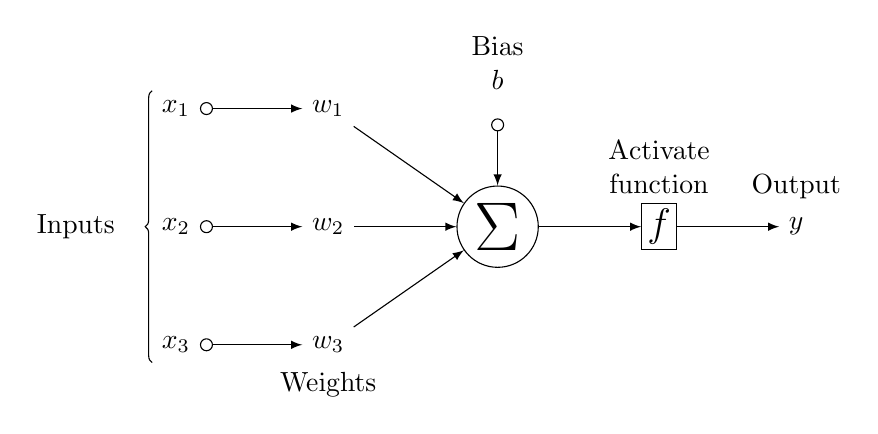
\begin{tikzpicture}[
init/.style={
	draw,
	circle,
	inner sep=2pt,
	font=\Huge,
	join = by -latex
},
squa/.style={
	draw,
	inner sep=2pt,
	font=\Large,
	join = by -latex
},
start chain=2,node distance=13mm
]
\node[on chain=2] 
(x2) {$x_2$};
\node[on chain=2,join=by o-latex] 
{$w_2$};
\node[on chain=2,init] (sigma) 
{$\displaystyle\Sigma$};
\node[on chain=2,squa,label=above:{\parbox{2cm}{\centering Activate \\ function}}]   
{$f$};
\node[on chain=2,label=above:Output,join=by -latex] 
{$y$};
\begin{scope}[start chain=1]
\node[on chain=1] at (0,1.5cm) 
(x1) {$x_1$};
\node[on chain=1,join=by o-latex] 
(w1) {$w_1$};
\end{scope}
\begin{scope}[start chain=3]
\node[on chain=3] at (0,-1.5cm) 
(x3) {$x_3$};
\node[on chain=3,label=below:Weights,join=by o-latex] 
(w3) {$w_3$};
\end{scope}
\node[label=above:\parbox{2cm}{\centering Bias \\ $b$}] at (sigma|-w1) (b) {};

\draw[-latex] (w1) -- (sigma);
\draw[-latex] (w3) -- (sigma);
\draw[o-latex] (b) -- (sigma);

\draw[decorate,decoration={brace,mirror}] (x1.north west) -- node[left=10pt] {Inputs} (x3.south west);
\end{tikzpicture}


\tikzset{%
	every neuron/.style={
		circle,
		draw,
		minimum size=1cm
	},
	neuron missing/.style={
		draw=none, 
		scale=4,
		text height=0.333cm,
		execute at begin node=\color{black}$\vdots$
	},
}

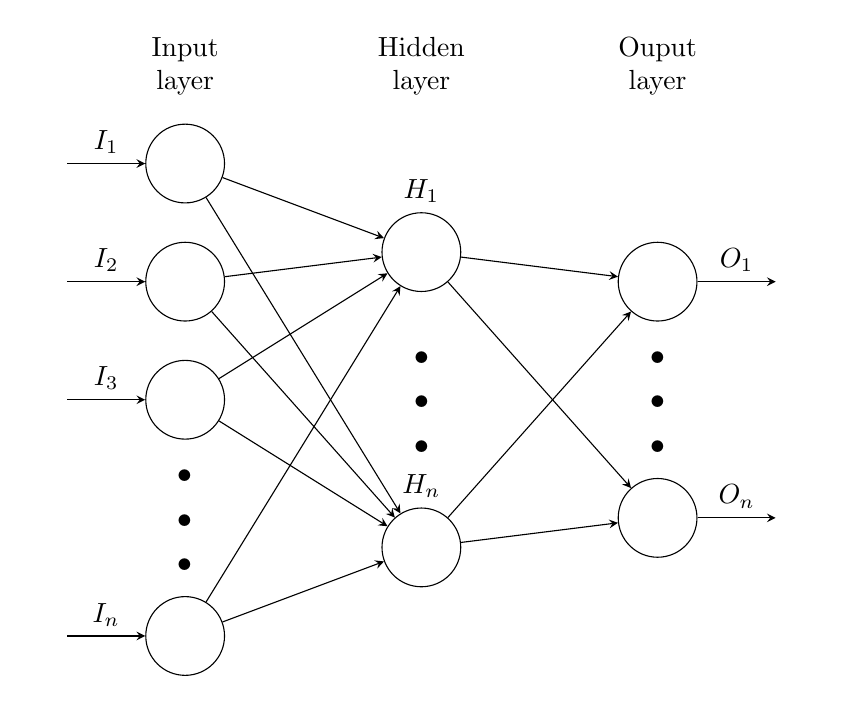
\begin{tikzpicture}[x=1.5cm, y=1.5cm, >=stealth]

\foreach \m/\l [count=\y] in {1,2,3,missing,4}
\node [every neuron/.try, neuron \m/.try] (input-\m) at (0,2.5-\y) {};

\foreach \m [count=\y] in {1,missing,2}
\node [every neuron/.try, neuron \m/.try ] (hidden-\m) at (2,2-\y*1.25) {};

\foreach \m [count=\y] in {1,missing,2}
\node [every neuron/.try, neuron \m/.try ] (output-\m) at (4,1.5-\y) {};

\foreach \l [count=\i] in {1,2,3,n}
\draw [<-] (input-\i) -- ++(-1,0)
node [above, midway] {$I_\l$};

\foreach \l [count=\i] in {1,n}
\node [above] at (hidden-\i.north) {$H_\l$};

\foreach \l [count=\i] in {1,n}
\draw [->] (output-\i) -- ++(1,0)
node [above, midway] {$O_\l$};

\foreach \i in {1,...,4}
\foreach \j in {1,...,2}
\draw [->] (input-\i) -- (hidden-\j);

\foreach \i in {1,...,2}
\foreach \j in {1,...,2}
\draw [->] (hidden-\i) -- (output-\j);

\foreach \l [count=\x from 0] in {Input, Hidden, Ouput}
\node [align=center, above] at (\x*2,2) {\l \\ layer};

\end{tikzpicture}

%\section{Title of the first subchapter of the first chapter}

